%==============================================================================
\chapter{Theory}
\label{sec:theory}
%==============================================================================

In this chapter, the theoretical background of this thesis will be discussed
in detail. This covers both physics as well as the techniques used for data
analysis. In the physics part, we will concentrate on neutrinos and their
properties and interactions, with special emphasis on neutrino oscillations.
The analysis part will describe the Fisher Information Matrix as a tool to
efficiently characterise a multi-dimensional likelihood landscape.

%==============================================================================
\section{Neutrinos in the Standard Model}
\label{sec:nus}
%==============================================================================


\subsection{Standard Model in a Nutshell}
\label{sec:NusInSM}

In the Standard Model of Particle Physics, or just Standard Model, the current
theories of the electroweak and strong interactions are combined
\cite{SMGlashow, SMWeinberg, SMSalam, SMtHooft}, for an overview see e.g.\
\cite{SMtextbook}. It is a quantum field theory of the fundamental interactions
and particles relevant on the scales that are accessible for particle physics
experiments.

\begin{figure}
\centering
  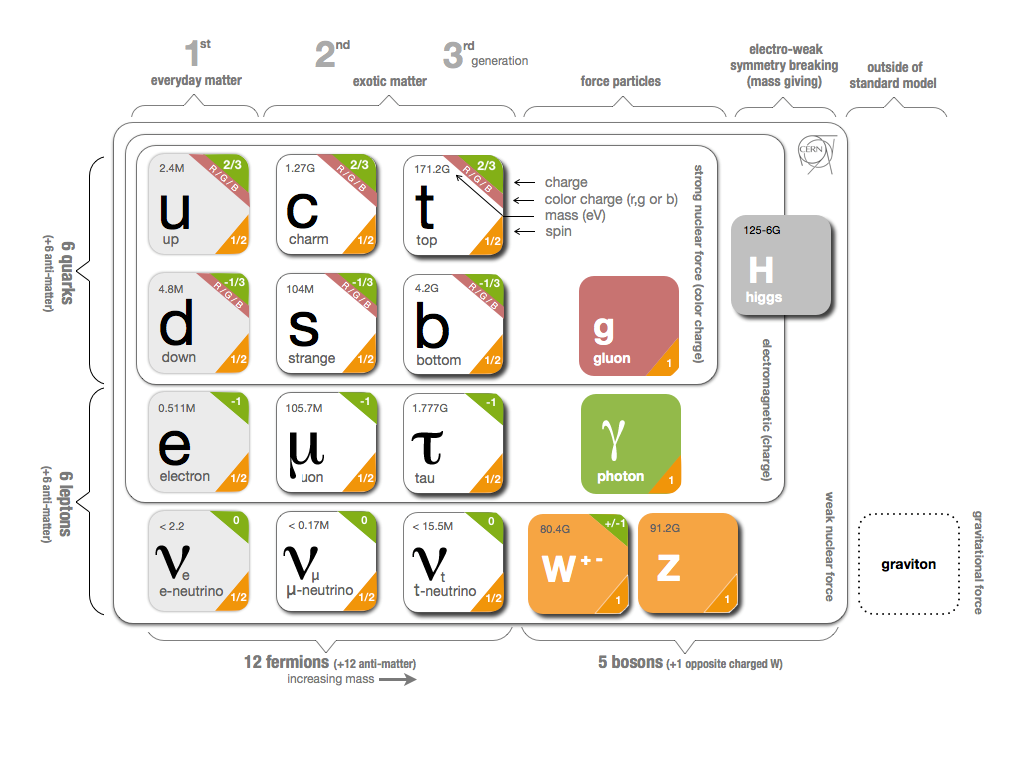
\includegraphics[width=0.8\textwidth]{Standard_model_infographic}
\caption{The fundamental particles in the Standard Model \cite{SMchart}.}
\label{fig:SMchart}
\end{figure}

The particles, listed in Fig.~\ref{fig:SMchart} can be divided in two classes:
fermions with an intrinsic spin of 1/2 make up everything that is usually called
``matter'', and exchange bosons with integer (1 in most cases) spin that convey
the interactions and couple to the respective charge. Formally, the bosons are
the generators of the gauge symmetry group of the particular interaction.

This means that the strong force, which obeys a \emph{SU(3)} symmetry, has eight
generators that are represented by eight gluons $g$. The gluons couple to the
strong charge which is usually referred to as ``colour''. Since it has the
largest coupling constant, the strong interaction is dominant whenever a
colour charge is present. However colour is ``confined'', i.e. free particles
must not have a net colour. This means that any coloured particles have to be
bound inside a compound object at all times. Also, the range of the strong
interaction is limited to about the size of a nucleus since the gluons are
coloured themselves and hence self-coupling.

About two orders of magnitude weaker is the electromagnetic interaction.
According to its \emph{U(1)} symmetry, it has only one exchange boson, the
photon $\gamma$, coupling to the electrical charge. It is massless and
electrically neutral, hence the electromagnetic interaction is not restricted
in range. This and the fact that there is no confinement on the electrical
charge mean that on macroscopic scales electromagnetic phenomena are dominant.

At low energies, the effective coupling constant of the weak interaction is
another three orders below the electromagnetic one. From its \emph{SU(2)}
symmetry originate three exchange bosons, $W^\pm$ and $Z^0$ with masses of
about 90\,MeV limiting its range to the subatomic scale. However with increasing
energy, the mass of the gauge bosons becomes more and more negligible and the
effective coupling rises. Above the electroweak unification at about 100\,GeV,
the weak and electromagnetic interactions can be described by one unified
theory, whose existence is also hinted to by the fact that the weak gauge
bosons are electrically charged.

Their masses arise from another spontaneously
broken local \emph{SU(2)}$\times$\emph{U(1)} symmetry of the so-called
Higgs\footnote{After Peter Higgs, who, together with others, laid the
foundations of this theory in the 1960's \cite{Higgs, BroutEnglert}.} field.
After breaking, the generators of the \emph{SU(2)} part mix with the weak
bosons, giving them mass, while the generator of the remaining \emph{U(1)} can
be observed as the only scalar gauge boson, the Higgs boson. The Higgs boson
was the last fundamental particle of the standard model to be detected, its
discovery was claimed by the ATLAS and CMS collaborations in 2012
\cite{AtlasHiggs, CMSHiggs}.

The other group of fundamental particles are the fermions (and their
corresponding antiparticles). They can be divided again into two subclasses: the
six quarks $u,\ d,\ c,\ s,\ t$, and $b$, which obey all forces and---being
coloured---are confined, so that no free quarks can be found in nature. Bound
quarks are making up baryons, like protons and neutrons, consisting of three
quarks, and unstable mesons, which consist of a quark and an antiquark, like
pions. Baryons and mesons, together called hadrons, are the only free particles
participating in the strong interaction, since they contain coloured quarks,
although not being coloured themselves.

The second subclass are the leptons, the three charged leptons $e$, $\mu$, and
$\tau$, as well as the corresponding (neutral) neutrinos \nue, \numu, and
\nutau. The charged leptons interact predominantly electromagnetically, most
prominently electrons are bound to nuclei via electrical attraction. However
the decay of $\mu$ and $\tau$ is---like every flavour-changing process---a weak
interaction. The electron as the lightest charged lepton has to be stable due
to conservation of energy and charge.

Since neutrinos are neither coloured nor electrically charged, they only
interact weakly. This means that they are very hard to detect directly. In
fact, their existence had already been suggested in 1930 by Wolfgang Pauli as a
solution for the problem of missing energy in radioactive $\beta$ decays
\cite{PauliBeta}. However the first direct detection of (electron) neutrinos,
\nue, from a nuclear reactor was achieved only in 1956 in the so-called
Cowan-Reines experiment \cite{CowanReines}. The existence of a second neutrino,
the muon neutrino \numu, was established few years later in 1962 from the study
of charged pion decays \cite{NuMuDiscovery}. The third neutrino, the \nutau,
was finally discovered directly by the DONUT experiment in 2001 in the decay of
$D_S$ mesons into \nutaubar and $\tau$, which again decay into \nutau and other
leptons \cite{DONUT}.

In addition to having neither colour nor electrical charge, the standard model
also predicts that neutrinos are massless. Thus the observation of neutrino
oscillations by the Super-Kamiokande experiment in 1998\footnote{Hints of
neutrino oscillations had already been observed in the 1960's
\cite{DaviesNuOsc}, but were widely refused by the scientific community.}
\cite{SuperKosc} gained much attention, this being the first detection of
physics beyond the standard model.

The term ``neutrino oscillations'' describes the phenomenon that neutrinos,
when propagating over macroscopic distances, can change their flavour
eigenstate on the way between production detection. The details of this effect
will be described in Sec.~\ref{sec:osc}. However it can only occur when there
are different mass eigenstates available for the neutrinos, meaning that only
one of them---if any---can have mass zero, while the others must correspond to
finite mass.

Since their first observation, neutrino oscillations have been a field of
intensive research. After establishing all oscillation channels, nowadays the
precise measurement of the parameters that characterise the oscillation is in
the focus. The planned PINGU experiment (see Sec.~\ref{sec:PINGU}), whose
simulation is the main topic of this thesis, is aimed to reach unprecedented
accuracy in measuring the parameters \thet{23} and \dm{31}.


\subsection{Neutrino Sources}
\label{sec:NuSources}

As discussed above, neutrinos do not participate in the strong and
electromagnetic interaction, leaving only weak processes for them to be created
or detected. On the other hand, neutrinos are produced in nearly every weak
interaction, making them a very common particle that can stem from a variety of
different sources in very different energy ranges.

\subsubsection{Natural Radioactivity}
On Earth, the most common source is the $\beta$ decay of natural radionuclides.
Depending on the type of the decay ($\beta^+$ or $\beta^-$), an electron
(anti-) neutrino is emitted along with the charged lepton. The general
equations read:
\begin{eqnarray}
 \beta^+: & ^A_Z\mathrm{X} & \to\quad  ^A_{Z-1}\mathrm{Y} + e^+ + \nue \\
 \beta^-: & ^A_Z\mathrm{X} & \to\quad  ^A_{Z+1}\mathrm{Y} + e^- + \nuebar
\end{eqnarray}
Examples for typical $\beta$ emitters are $^{40}$K (both $\beta^+$ and
$\beta^-$) and intermediate products from the decay chains of $^{232}$Th or
$^{238}$U ($\beta^-$), the neutrino energies are usually on the scale of few
MeV.

In fact, the $\beta$ decay was the original reason to propose the existence of
the then un-detectable neutrino. Since only the daughter nucleus and the
charged lepton were visible as decay products, the process seemed to be a
two-body decay. This means that the energies of the decay products are exactly
determined from kinematics and hence the emitted electrons or positrons would
be monoenergetic. Observations showed, however, a broad spectrum in energy
instead of a single line. Without violating the conservation of energy, this
can only be achieved if a third particle is produced in the process, which is
electrically neutral but can carry away energy and momentum. 

On the subatomic level, in a $\beta^+$ decay one proton inside a nucleus emits a
virtual $W^+$ boson, turning an $u$ into a $d$ quark, and becomes a neutron.
During a $\beta^-$ decay, the opposite happens via the emission of a $W^-$, as
shown in Fig.~\ref{fig:beta_minus}. The $W$ boson subsequently decays into a
charged lepton and a neutrino.

\begin{figure}
 \centering
 \begin{fmffile}{beta_minus}
 \begin{fmfgraph*}(80,50) \fmfpen{thin}
 \fmfstraight
  \fmfleft{i0,i1,i2,i3,i41,i42,i5,i51,i6}
  \fmfright{o0,o1,o2,o3,o41,o42,o5,051,o6}
  \fmf{fermion}{i0,o0}
  \fmflabel{$u$}{i0}
  \fmflabel{$u$}{o0}
  \fmf{fermion}{i1,o1}
  \fmflabel{$d$}{i1}
  \fmflabel{$d$}{o1}
  \fmf{fermion}{i2,v1,o2}
  \fmflabel{$d$}{i2}
  \fmflabel{$u$}{o2}
  \fmffreeze
  \fmf{fermion}{o5,v2,o6}
  \fmflabel{$e^-$}{o6}
  \fmflabel{\nuebar}{o5}
  \fmf{dashes,lab=$W^-$,l.side=left,tension=1.5}{v1,v2}
 \end{fmfgraph*}
 \end{fmffile}
 \write18{mpost beta_minus}
\caption{Feynman diagram of a $\beta^-$ decay}
\label{fig:beta_minus}
\end{figure}

% TODO: say something about 0n2b decay?


\subsubsection{Nuclear Reactors}

In nuclear reactors, the controlled fission of heavy elements is used for the
generation of electrical power. The intermediate products of these nuclear
fissions are unstable isotopes that usually have a large surplus of neutrons
compared to a stable configuration. These unstable nuclides undergo a series of
$\beta^-$ decays until they they reach a stable ratio of proton and neutron
numbers.

Since in each of those $\beta$ decays neutrinos are emitted, a nuclear reactor
provides a strong and steady flux of \nuebar, which can be monitored via the
thermal power of the reactor. This makes reactor neutrinos a popular target for
experiments, especially for the study of neutrino oscillations. The main
challenge in such experiments is the accurate modelling of the neutrino energy
spectrum, which is the sum of the spectra of all of the different $\beta$
decays in the decay chain. Even though there are very elaborate flux models
available, there might still be components unaccounted for, resulting in
unexpected features in the measured neutrino flux \cite{RENO_5MeV}.


\subsubsection{Neutrino Beams}

Another artificial source of neutrinos, but somewhat higher in energy
(typically at a few GeV) are neutrino beams. Since the neutral neutrinos cannot
be accelerated directly, usually a high-energy, high-intensity proton beam is
aimed at a target in which it produces mesons, mostly pions and kaons, in whose
subsequent decay neutrinos are produced \cite{NuBeams}:
\begin{eqnarray}
 \pi^+ & \to & \mu^+ + \numu \\
 \pi^- & \to & \mu^- + \numubar
\end{eqnarray}

Such beams are the source of neutrinos that can be controlled best in terms of
energy and intensity, making them a preferred choice for precision experiments
such as measurements of neutrino cross-sections. However they are very expensive
to build and operate in contrast to natural sources or nuclear reactors, the
latter usually being operated by commercial power suppliers.


\subsubsection{Solar Neutrinos}

In terms of total flux, the strongest source of neutrinos on Earth is the Sun.
In its interior, hydrogen is fused to helium mostly in the so-called pp
chain\footnote{Other fusion processes such as the CNO cycle and the production
of heavier elements are strongly suppressed since they need extremely high
pressures that the Sun cannot supply due to its comparatively low mass.},
producing the energy that powers the Sun's radiation\cite{RolfsRodney}.

\begin{figure}
\centering
  \subfloat[The different branches of the pp chain.
    ``Lost'' energy is not dissipated into the Sun, but carried away by
    neutrinos. \label{fig:pp_network}]
    {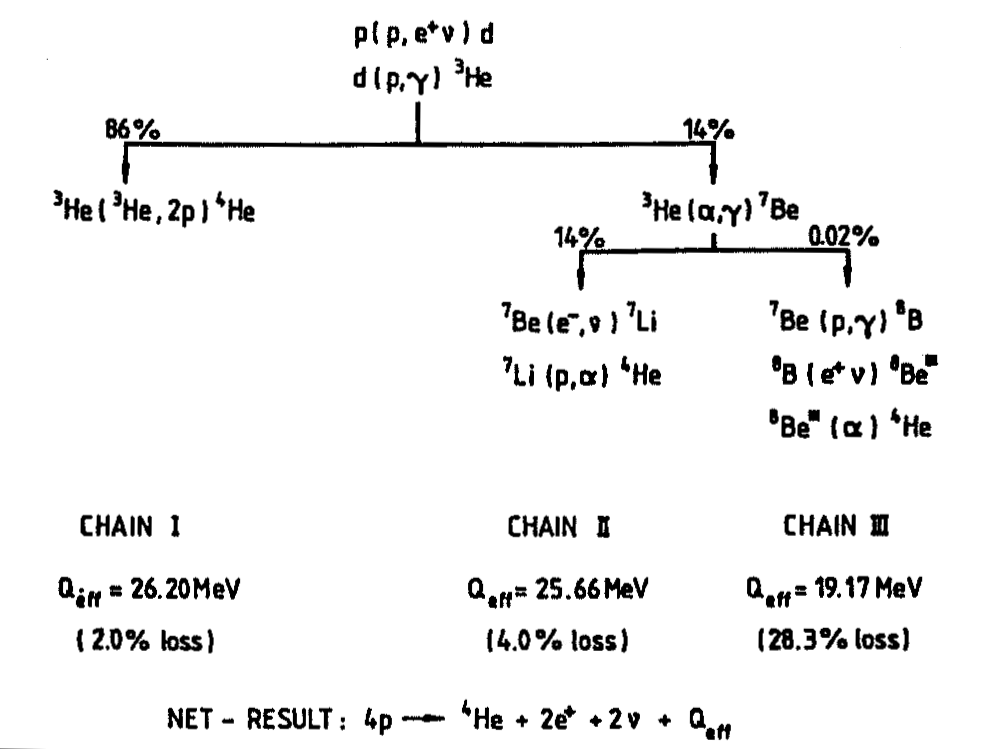
\includegraphics[width=0.45\textwidth]{pp_chain}}\qquad
  \subfloat[The solar neutrino spectrum from the pp chain.
    The neutrino fluxes are in units of cm$^{-2}$\,s$^{-1}$\,MeV$^{-1}$ for
    continuous and cm$^{-2}$\,s$^{-1}$ for discrete components.
    \label{fig:solar_nu_spectrum}]
    {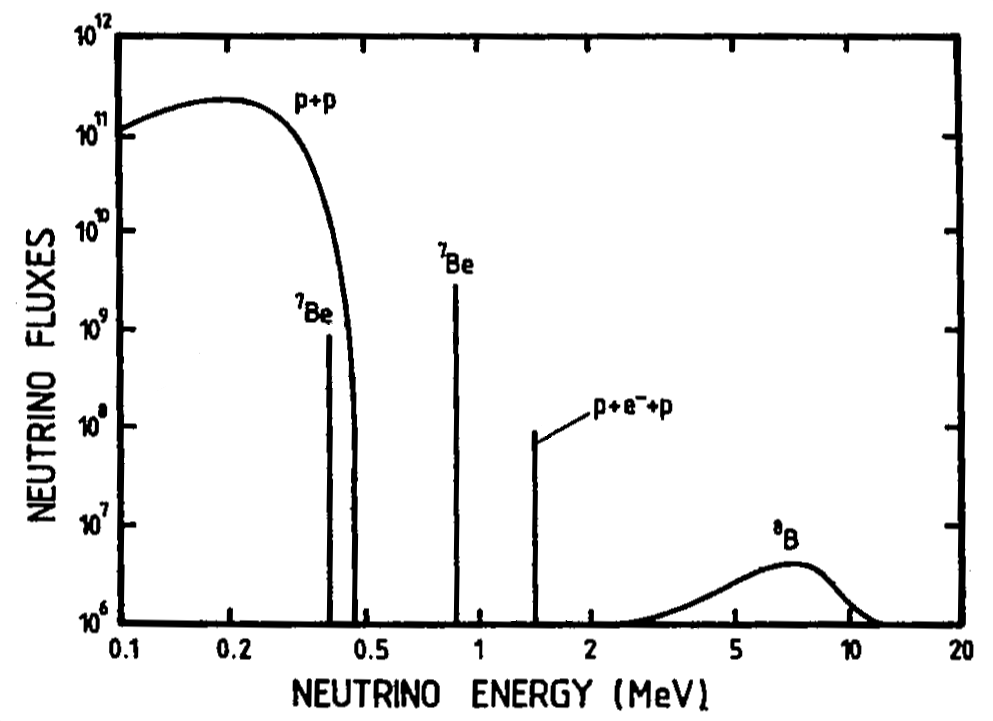
\includegraphics[width=0.45\textwidth]{solar_nu_spectrum}}
  \caption{The reactions and resulting neutrino spectrum of the solar pp chain.
    Figures adopted from \cite{RolfsRodney}.}
\label{fig:solar_nus}
\end{figure}

Effectively, this is carried out via the reaction
\begin{equation}
 4 p \to\ ^4_2\mathrm{He} + 2 e^+ + 2 \nue + 26.73\,\mathrm{MeV}\quad.
\end{equation}
In reality, this will not occur in a single step since it is a weak interaction
(as neutrinos are produced in its course) with a correspondingly small
cross-section which in addition has to overcome the Coulomb repulsion of the
four protons. Instead the fusion process involves several intermediate stages,
the first of which is the fusion of two protons to a deuteron,
\begin{equation}
 p + p \to\ d + e^+ + \nue\quad,
\end{equation}
releasing 0.42\,MeV of energy carried by the (subsequently annihilating)
positron and the so-called pp neutrino. The low Q value along with the
aforementioned low cross-section and Coulomb repulsion are the reason for the
long lifetime of free protons inside the Sun\footnote{And hence also the
long lifetime of the Sun itself}---it takes them an average of about $10^{10}$
years to fuse to deuterium. A competing, but even more improbable reaction is
the pep process, where an electron is involved directly in the fusion and no
positron is produced:
\begin{equation}
 p + e^- + p \to\ d + \nue
\end{equation}
Since there are only two particles in the final state, the produced neutrinos
are monoenergetic at 1.44\,MeV. Once a deuteron is produced, it quickly (YYY\,s)
merges with another proton to $^3_2\mathrm{He}$ and emits a photon.

At this stage, the pp chain divides into three different branches (see
Fig.~\ref{fig:pp_network}). In the main branch, ppI, two $^3_2\mathrm{He}$
nuclei fuse to $^4_2\mathrm{He}$, also called an $\alpha$ particle, and two
protons that can then enter the pp chain again. However in terms of neutrinos,
the two subdominant branches ppII and ppIII are much more interesting,
especially since the pep and pp neutrinos, who make up the main part of the
solar neutrinos, are very low in energy and thus difficult to detect.

If a $^3_2\mathrm{He}$ does not fuse with another $^3_2\mathrm{He}$, but with
a $^4_2\mathrm{He}$ instead, $^7_4\mathrm{Be}$ is formed. In most cases, this
will then capture an electron to produce $^7_3\mathrm{Li}$ under the emission
of a neutrino in the ppII branch:
\begin{equation}
 ^7_4\mathrm{Be} + e^- \to\ ^7_3\mathrm{Li} + \nue
\end{equation}
These so-called $^7$Be neutrinos have an energy of 0.86\,MeV. Due to this high
energy and their rather high flux portion of about 14\,\%, they were targeted
in the first detection of solar neutrinos \cite{DaviesNuOsc}. The
$^7_3\mathrm{Li}$ finally catches another proton to form two $^4_2\mathrm{He}$
nuclei.

Sometimes, the $^7_4\mathrm{Be}$ reacts with a proton rather than an electron
(ppIII branch) and forms $^8_5\mathrm{B}$, which is a $\beta^+$ emitter with a
half-life of 0.77\,s \cite{Nuklidkarte}. Although their flux is very low, the
very high Q-value of 14.1\,MeV of this decay makes the so-called $^8$B a
favourable target for the search for solar neutrinos.

The excited $^8_4\mathrm{Be}$ created in the decay
\begin{equation}
 ^8_5\mathrm{B} \to\ ^8_4\mathrm{Be^*} + e^+ + \nue
\end{equation}
will then further decay into two $\alpha$ particles immediately.


\subsubsection{Atmospheric Neutrinos}
\label{sec:AtmNus}

Several orders of magnitude higher in energy are neutrinos that are created in
the interaction of high-energy charged particles with atoms in the Earth's
atmosphere. During the past decades, the spectrum of these particles, the 
so-called cosmic radiation, has been measured in great detail over many orders
of magnitude. Although it covers such a wide range in energy and flux, it shows
almost no features and can be described by a simple power law with a spectral
index of $\gamma=-2.7$, softening to $\gamma=-3.0$ at the so-called ``knee'' at
a few PeV and turning back to $\gamma=-2.7$ at the ``ankle'' at the highest
energies \cite{CosmRad}.

\begin{figure}
\centering
  \subfloat[The all particle spectrum of the charged cosmic radiation. Figure
    taken from \cite{CosmRaySpec}. \label{fig:CosmRaySpec}]
    {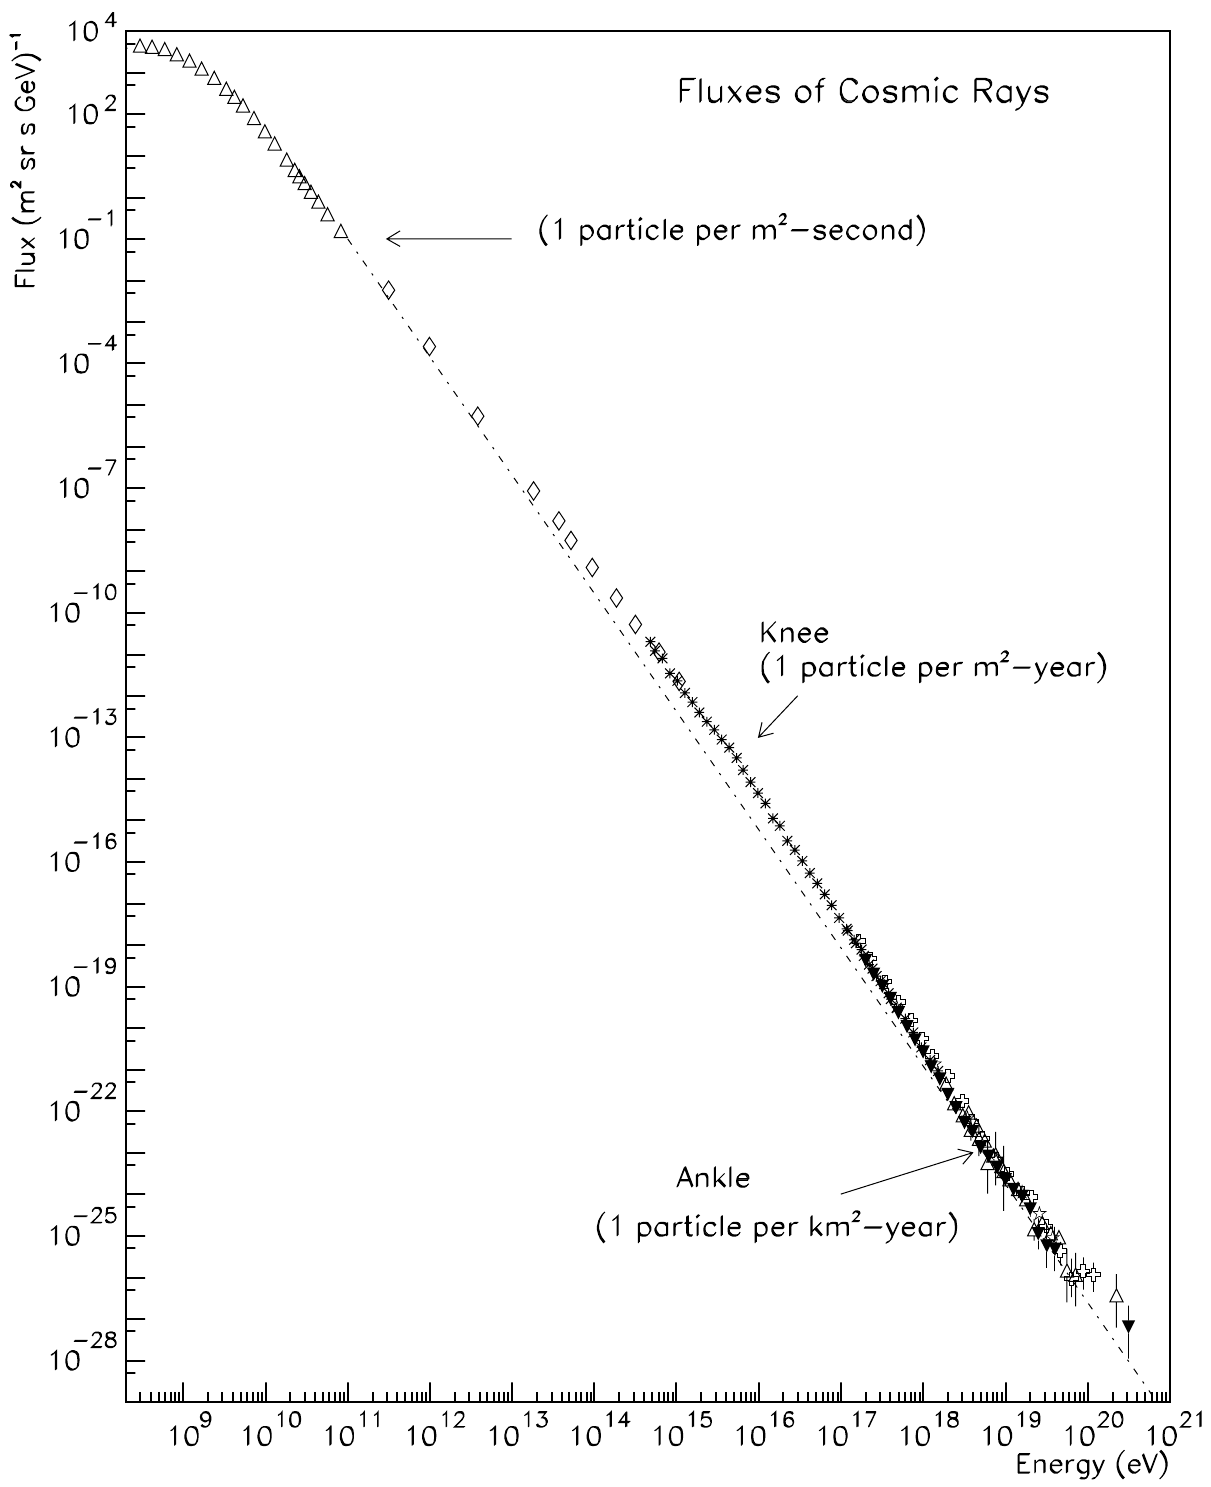
\includegraphics[height=7cm]{CosmicRaySpectrum}}\qquad
  \subfloat[The atmospheric flux of electron and muon neutrinos.
    Predictions for the conventional flux are from \cite{Honda2007} (solid
    lines) and \cite{Bartol} (dashed), the band for the prompt flux is
    according to \cite{PromptFlux}. Figure taken from \cite{IC_AtmCscd}.
    \label{fig:AtmFlux}]
    {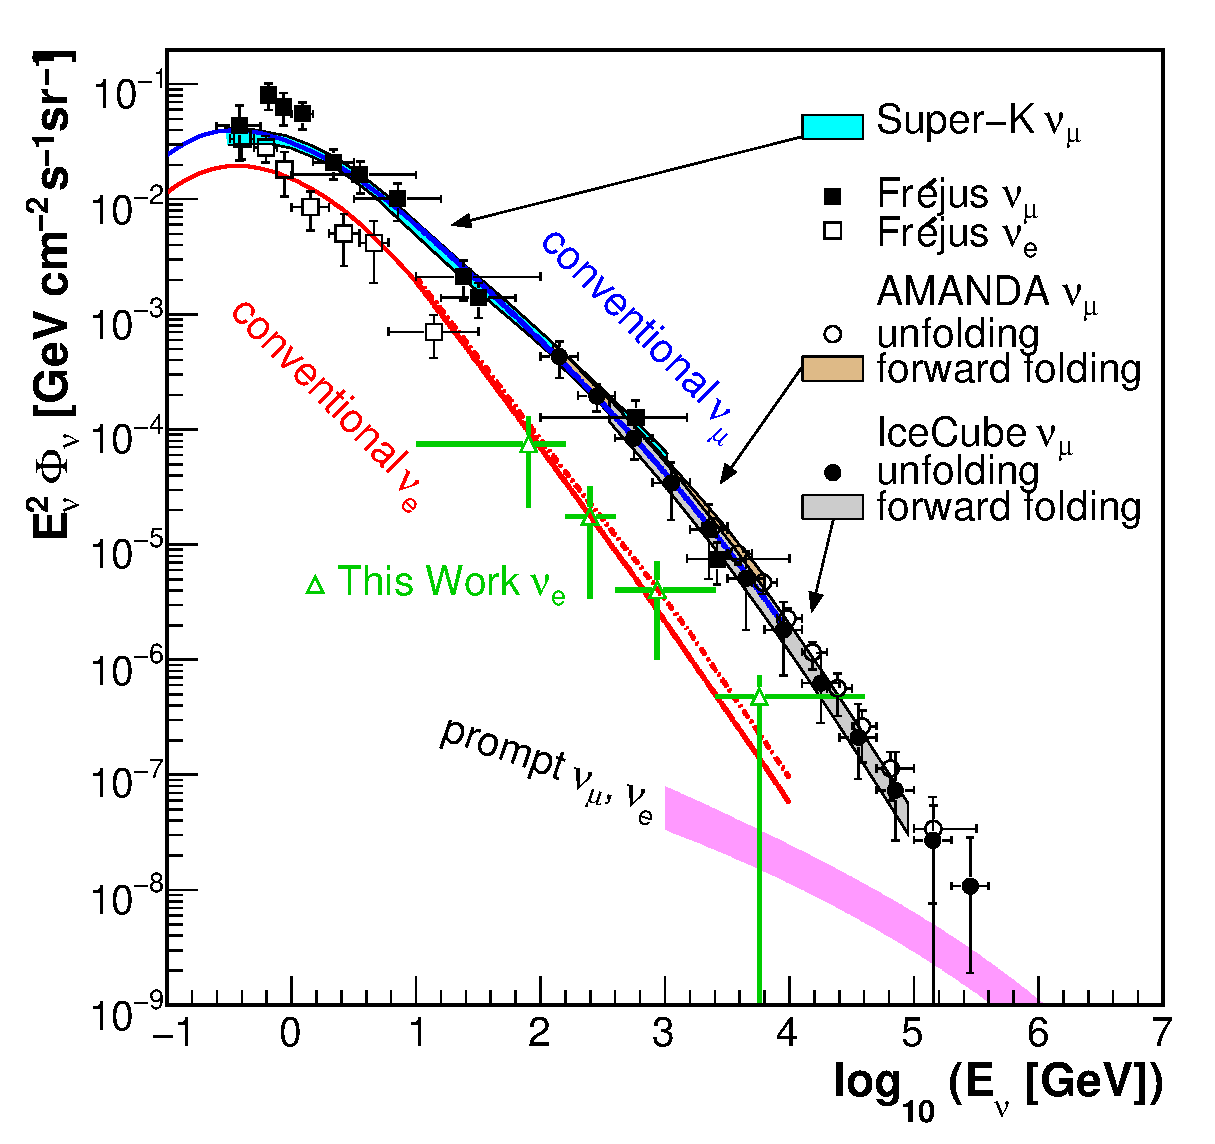
\includegraphics[height=7cm]{AtmFlux}}
  \caption{Spectra of the cosmic radiation at Earth and the resulting
    atmospheric neutrino spectrum.}
\label{fig:cosmic_rays_atm_nus}
\end{figure}

The origin of the cosmic radiation is not fully established yet. However it is
commonly assumed that the particles are accelerated in non-thermal processes,
usually moving shock fronts, that develop in extreme astrophysical environments.
This mechanism is known as Fermi acceleration \cite{FermiAcc}. 
Candidates for the acceleration sites are both galactic sources, such as
supernova remnants, as well as extragalactic ones like gamma ray bursts or
active galaxies. Due to their small size and rather low energy density, galactic
sources are believed to dominate the low-energy part of the spectrum in the GeV
to TeV regime, while the extragalactic contribution takes over at the knee
region.

When such a high energy particle hits the Earth's atmosphere, it interacts with
a nucleus in the air (usually nitrogen or oxygen) in a so-called deep-inelastic
scattering process. Since the energy of the incoming particle is far beyond all
binding energies in the nucleus, it is completely disrupted. From the fragments
of the nucleus that are still highly energetic, a shower of secondary particles
develops, that then travels down to Earth.

Main components of these particle showers are muons and pions. Both particles
are relatively short-lived\footnote{$\tau_\mu = 2.2 \times 10^{-6}$\,s and
$\tau_\pi = 2.6 \times 10^{-8}$\,s \cite{PDG}} and produce neutrinos in their
decay:
\begin{eqnarray}
 \pi^\pm &\to\ & \mu^\pm + \numu(\numubar) \\
 \mu^\pm &\to\ & e^\pm + \nue(\nuebar) + \numubar(\numu)
 \label{eqn:pi_decay}
\end{eqnarray}
As one can see from the above equations, these so-called conventional
atmospheric neutrinos coming mostly from pion decay have a flavour ratio of
$\overset{(-)}{\numu}:\overset{(-)}{\nue} = 2:1$.

Their energy spectrum is linked to the primary spectrum of cosmic rays since the
secondary pions and muons follow the primary energy distribution directly. Thus
being highly relativistic, their livetime is Lorentz boosted by a factor $\gamma
\propto E$. This means that the higher the pion's (or muon's) energy, the higher
its probability \emph{not} to decay into neutrinos in-flight but reach the
Earth's surface and interact there, producing another shower of much less
energetic particles. Hence the spectrum of conventional atmospheric neutrinos
is suppressed roughly by a factor of $1/E$ with respect to the primary cosmic
ray distribution.

For a more precise calculation, details of high-energy proton interactions and
the geomagnetic field have to be taken into account \cite{Honda2007, Bartol}. As
shown in Fig.~\ref{fig:cosmic_rays_atm_nus}, these predictions show good
agreement with measurements.

Another predicted, but not yet observed component of the atmospheric neutrino
flux are the so-called prompt neutrinos. They originate from charmed mesons,
mostly kaons, that are rarely produced in cosmic ray induced air showers as
well. Since these are so short-lived that they always decay in-flight
(``promptly'') despite of their relativistic boost, their energy spectrum
is the same as the primary one and thus harder than the conventional component,
but with a much smaller normalisation.

\subsubsection{Supernova Neutrinos}
% TODO: mention them?

\subsubsection{Astrophysical Neutrinos}

The highest energy neutrinos are the so-called astrophysical ones. They are  
assumed to be produced at similar sites as the cosmic radiation, i.\,e.\ in 
highly energetic shock fronts. There, $\Delta$ resonances are generated in the 
collision of protons and high-energy photons, producing pions in their decay:
\begin{equation}
 p + \gamma \to \Delta^+ \to n + \pi^+\ (p + \pi^0)
\end{equation}
The pions then decay further into neutrinos as shown in (\ref{eqn:pi_decay}).

Since astrophysical neutrinos are produced in the same processes as cosmic 
rays, their fluxes are linked. The flux of cosmic rays has been measured in 
quite some detail over the recent decades \cite{CosmRaySpec}, hence an upper 
limit for the flux of astrophysical neutrinos can be derived that is 
independent of any model assumptions about the production sites \cite{WB_bound}.

The first actual astrophysical neutrino events have been recorded only recently 
by the IceCube neutrino telescope \cite{HESE, HESE_3yr}, making them the 
highest energy neutrinos ever observed. Although event statistics are still 
low, the flux seems to be very close to the predicted upper bound, meaning that 
the neutrino production efficiency is close to maximal. The spectral shape of 
the flux is compatible with a power law with an index of --2 and an exponential 
cut-off around a few PeV \cite{Lars_globalfit}.

\subsection{Detection of Neutrinos}

As already mentioned, neutrinos only interact with other particles in weak
processes. This means that the total cross-sections are typically low. So high
fluxes or large target volumes (or both) are needed to detect a seizable
number of neutrinos.

And even if these requirements are fulfilled, in most cases the neutrino signal
has to be recovered from below a background of dominant processes, whose rate
can be several orders of magnitude higher than the neutrino event rate.
Depending on the targeted energy range, the most common background processes are
inherent radioactivity of the surroundings and the detector itself at MeV
energies, and muons created in cosmic ray induced air showers which can
penetrate even strong shielding.

\subsubsection{Neutrino cross-sections}

\begin{figure}
 \centering
 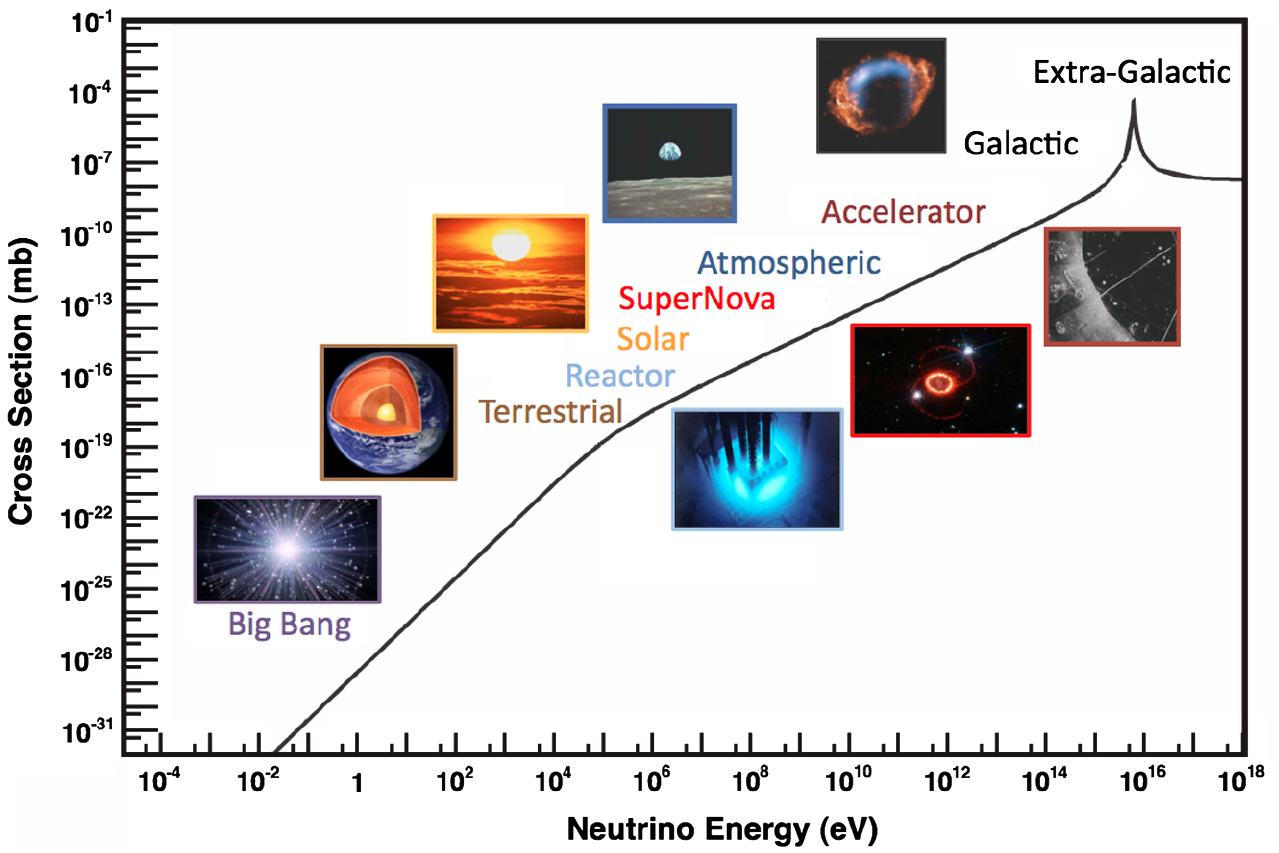
\includegraphics[width=0.7\textwidth]{NuXsec_fullrange}
\caption{Electroweak cross-section for $\nue e^- \to \nue e^-$ scattering
  on free electrons as a function of neutrino energy. Various neutrino sources
  are also shown at their respective energy scales. \cite{NuXsec_review}}
 \label{fig:nue_e_xsec}
\end{figure} 

The calculation and experimental testing of neutrino cross-sections has been a
field of extensive research over the past decades. On the experimental side,
the challenge is the smallness of the cross-sections. The key point on the
theoretical side is the calculation of the matrix elements associated with the
interaction of interest.

As an introductory example, we will look at neutrinos scattering off a free
lepton. Then the cross-section is \cite{NuXsec_review}
\begin{equation}
 \frac{d\sigma}{dq^2} = \frac{1}{16\pi} \frac{|\mathcal{M}^2|}{(s-m_e^2)^2}\ ,
\end{equation}
with $s$ and $q^2$ being the centre-of-mass energy and the four-momentum
transfer, respectively, assuming very small neutrino mass. In this case,
calculating the matrix element $|\mathcal{M}^2|$ is rather straightforward,
since only weak interactions between fundamental particles have to be
considered. The scattering process itself is the sum of a charged-current
($W^+$ exchange, CC) and a neutral current ($Z^0$ exchange, NC) contribution, as
shown in Fig.~\ref{fig:nue_e_CC}.

% TODO: Feynman graphs!
\begin{figure}
 \centering
 \begin{fmffile}{nue_e_CC}
 \parbox{50mm}{
  \begin{fmfgraph*}(40,30) \fmfpen{thin}
    \fmfstraight
    \fmfleft{i00,i0,i2,i3,i41,i42,i5,i51,i6,i1}
    \fmfright{o00,o0,o2,o3,o41,o42,o5,o51,o6,o1}
    \fmf{fermion}{i0,v0,o0}
    \fmflabel{$e^-$}{i0}
    \fmflabel{$\nue$}{o0}
    \fmf{fermion}{i1,v1,o1}
    \fmflabel{$\nu_f$}{i1}
    \fmflabel{$f^-$}{o1}
    \fmf{dashes,lab=$W$,l.side=left,tension=1.}{v0,v1}
  \end{fmfgraph*}
  } + \qquad \quad
 \parbox{50mm}{
  \begin{fmfgraph*}(40,30) \fmfpen{thin}
    \fmfstraight
    \fmfleft{i00,i0,i2,i3,i41,i42,i5,i51,i6,i1}
    \fmfright{o00,o0,o2,o3,o41,o42,o5,o51,o6,o1}
    \fmf{fermion}{i0,v0,o0}
    \fmflabel{$e^-$}{i0}
    \fmflabel{$f^-$}{o0}
    \fmf{fermion}{i1,v1,o1}
    \fmflabel{$\nu_f$}{i1}
    \fmflabel{$\nue$}{o1}
    \fmf{dashes,lab=$Z^0$,l.side=left,tension=1.}{v0,v1}
  \end{fmfgraph*}
 }
 \end{fmffile}
 \write18{mpost nue_e_CC}
 \caption{Feynman diagrams for the charged (left) and neutral (right) current
  contributions of $\nu_f\,e^- \to \nue\,f^-$ scattering.}
\label{fig:nue_e_CC}
\end{figure}

After converting from momentum transfer to the energy fraction $y$ carried by 
the outgoing lepton, $\frac{dq^2}{dy} = 2m_e E_\nu$, the charged current
cross-section for scattering off an electron is given by \cite{NuXsec_review}
\begin{equation}
 \frac{d\sigma}{dq^2}\bigg\rvert_\mathrm{CC} = \frac{2m_e G_F^2 E_\nu}{\pi}
  \left(1 - \frac{m_f^2 - m_e^2}{2m_e E_\nu}\right)\ ,
 \label{eqn:nue_e_xsec}
\end{equation}
where $E_\nu$ is the incoming neutrino energy, and $m_e$ and $m_f$ are the
masses of the electron and the outgoing fermion. The corresponding total
cross-section for $\nue e^- \to \nue e^-$ scattering is shown in
Fig.~\ref{fig:nue_e_xsec}. In case that $m_f$ can be neglected compared to the
neutrino energy, the above can be integrated to give a simple expression for
the total cross-section:
\begin{equation}
 \sigma \simeq \frac{2m_e G_F^2 E_\nu}{\pi} = \frac{G_F^2 s}{\pi}
\end{equation}
In Fig.~\ref{fig:nue_e_xsec}, this corresponds to the regime above about
$10^7$\,eV, well above the electron mass. The sharp peak at $\sim 10^{16}$\,eV
is the so-called Glashow resonance, where the centre-of-mass energy is
comparable to the $W$ boson mass, enabling resonant production of real $W^-$
bosons and hence causing a strong enhancement of the cross-section.

% FIXME: also write down nubar  and NC cross-section?

When looking at other scattering processes, the principles of deriving the
cross-section remain the same. However the kinematic part is subject to change,
mostly due to different angular momentum states, and of course the matrix
elements depend strongly on the respective target. For non-fundamental targets,
form factors describing their internal charge distribution have to be taken
into account as well.

In general, the cross-section for hadronic interactions are much larger than the
leptonic ones (e.\,g.\ neutrino-electron scatting as discussed above) due to the
larger target masses. This means that for conventional target consisting of
atoms with a nucleus and an electron hull, a neutrino is much more likely to
interact with the nuclei than with the shell electrons.

\subsubsection{Neutrino interactions with hadrons at the GeV scale}

\begin{figure}
\centering
  \subfloat
    {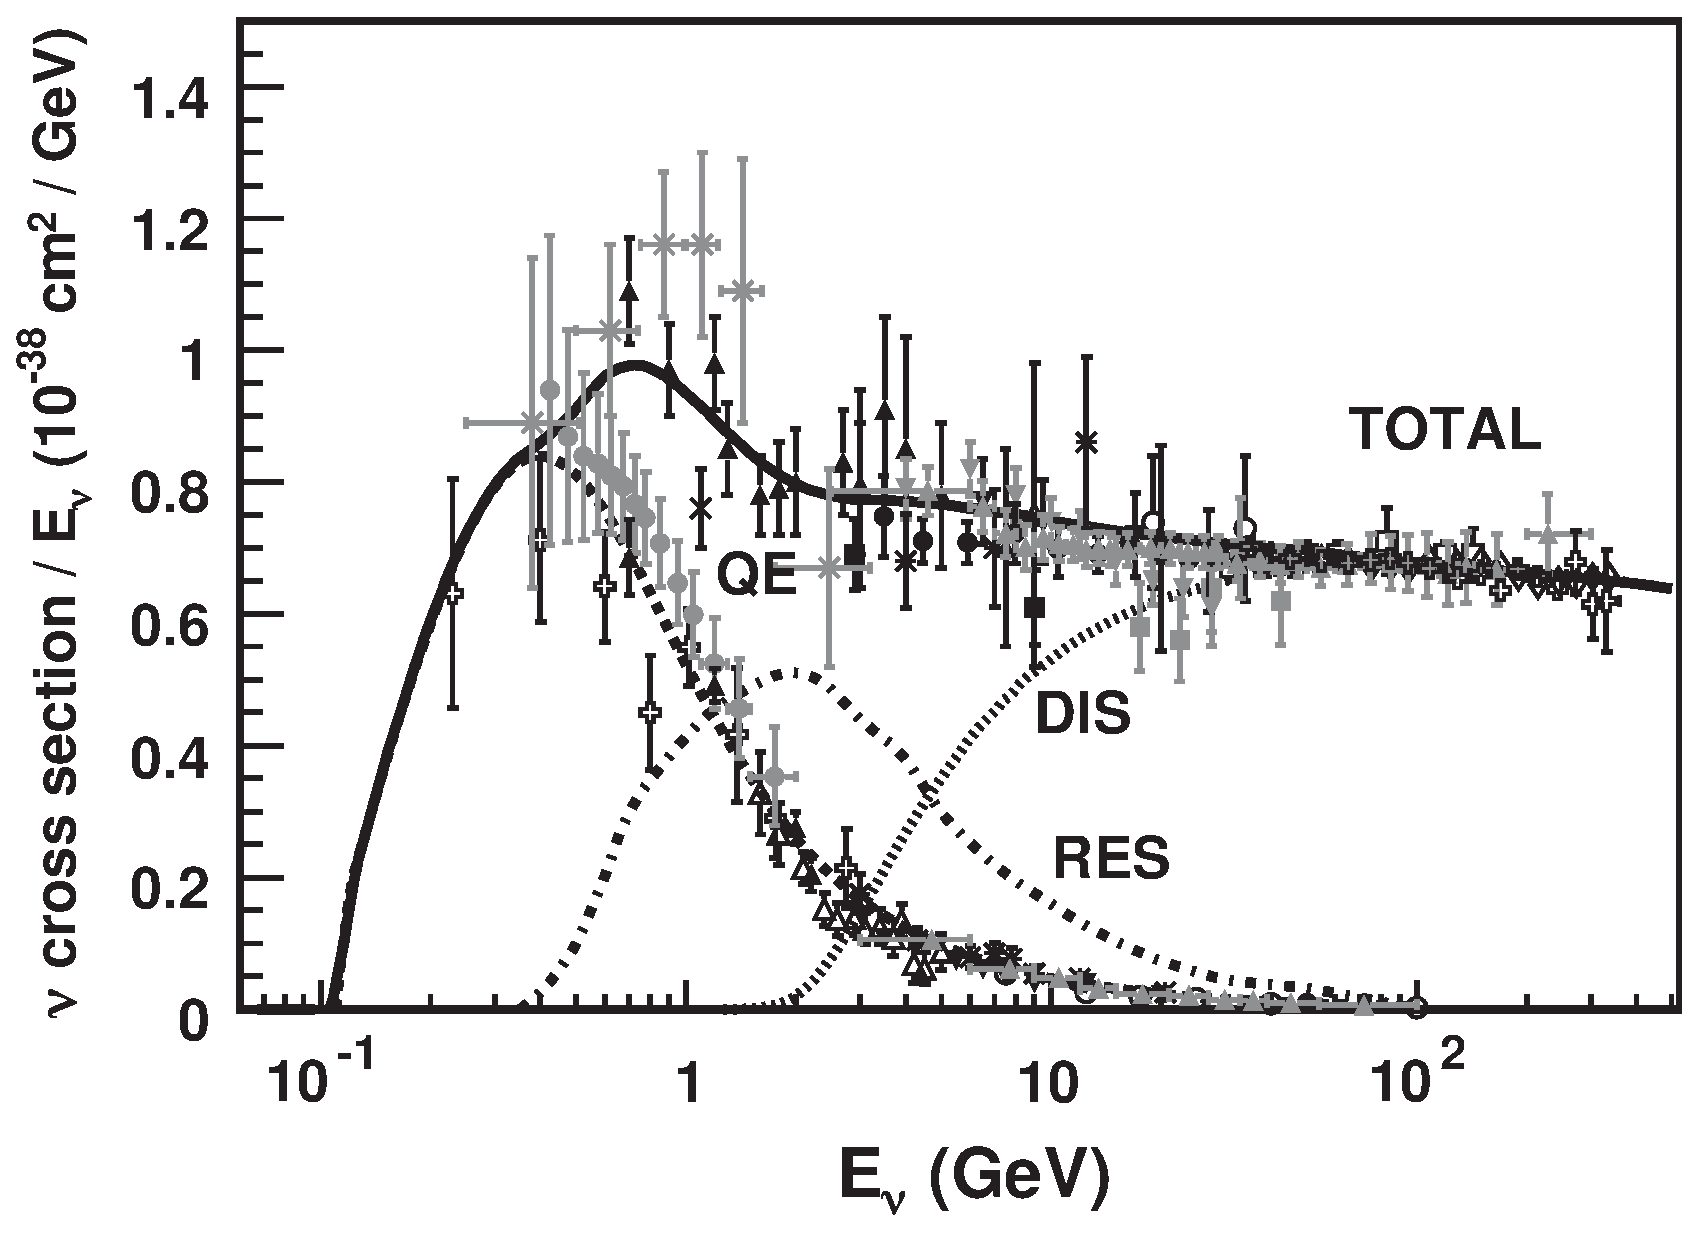
\includegraphics[width=7cm]{nu_N_xsec}}\qquad
  \subfloat
    {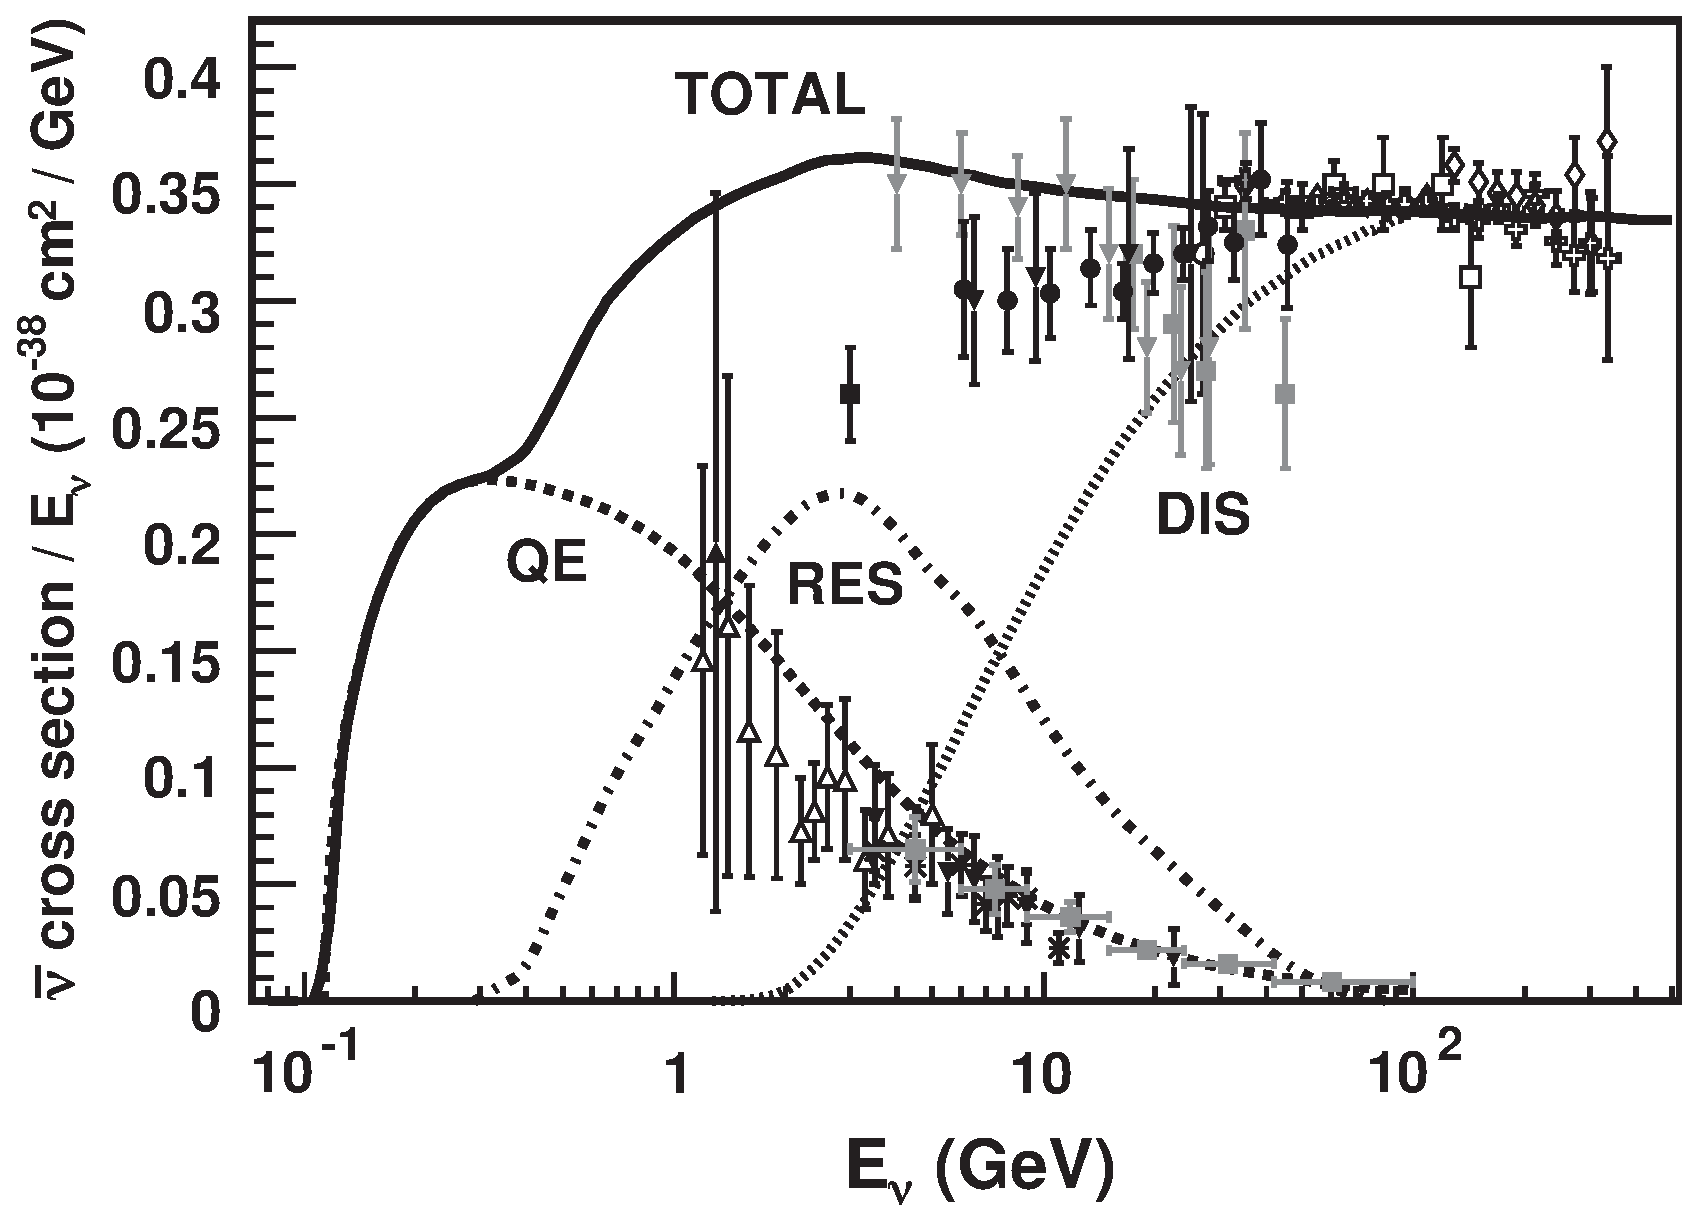
\includegraphics[width=7cm]{nubar_N_xsec}}
  \caption{Total CC cross-section for neutrino (left) and antineutrino
   (right) cross-section for an isoscalar nucleon, $N=(p+n)/2$, divided by the
   neutrino energy and plotted as a function of energy. Shown are data from
   various experiments and predictions for the quasi-elastic (QE), resonance
   (RES), and deep inelastic (DIS) contributions \cite{NuXsec_review}.}
\label{fig:NuXsec_GeV}
\end{figure}

For the scope of this thesis, the most interesting energy regime is the low GeV
scale, especially the range of $1 - 50$\,GeV. Here the cross-section for
neutrino interactions with nuclei is quite complex to describe, as several
distinct processes (shown in Fig.~\ref{fig:NuXsec_GeV}) have to be considered
for the scattering:
\begin{itemize}
 \item \emph{Quasi-elastic scattering:} At rather low energies, the neutrino
    scatters off an entire nucleon, removing it (possibly together with other
    nucleons) from the nucleus. The free proton(s) or neutron(s) will then
    propagate through the surrounding medium until they have dissipated all
    their energy. These interactions range out quickly above about 10\,GeV.
 \item \emph{Resonance production:} At the range of about $1-3$\,GeV, the
    dominant process is the excitation of short-lived baryonic resonances
    (such as $\Delta^+$ or $N^*$) in the target nucleon. These resonances then
    decay to various final states producing nucleons and $\pi$ mesons.
 \item \emph{Deep inelastic scattering:} Above about 10\,GeV, the scattering
    neutrino has sufficient energy to resolve the quark structure of the
    nucleons. Then it scatters on a quark constituent rather than the whole
    nucleon. By this, the nucleon gets disrupted and an hadronic shower
    consisting of a variety of mesons forms from its remains.
\end{itemize}

Common to all these processes is that they have both a CC and a NC
contribution---similar to the scattering off electrons shown in
Fig.~\ref{fig:nue_e_CC}, only that the target is either a whole (for
quasi-elastic and resonant processes) or a quark inside a nucleon (deep
inelastic scattering).

\begin{figure}
 \centering
 \begin{fmffile}{nux_NC}
 \begin{fmfgraph*}(50,30) \fmfpen{thin}
 \fmfstraight
  \fmfleftn{i}{8}
  \fmfrightn{o}{8}
  \fmf{heavy}{i2,v1}
  \fmfv{decor.shape=circle,decor.filled=shaded}{v1}
  \fmf{vanilla}{v1,o2}
  \fmflabel{nucleus}{i2}
  \fmflabel{hadronic\ shower}{o2}
  \fmf{fermion}{i8,v2,o8}
  \fmflabel{$\nu$}{i8}
  \fmflabel{$\nu'$}{o8}
  \fmf{dashes,lab=$Z^0$,l.side=left,tension=1.5}{v1,v2}
  \fmffreeze
  \fmf{vanilla}{v1,o1}
  \fmf{vanilla}{v1,o3}
 \end{fmfgraph*}
 \end{fmffile}
 \write18{mpost nux_NC}
\caption{Neutral current interaction between a neutrino and a nucleus.}
\label{fig:nux_NC}
\end{figure}

From the detection point of view, this means that there are four classes of
events. The first are neutral current interactions of any neutrino flavour, as
shown in Fig.~\ref{fig:nux_NC}. In this case, we have in the final state the
scattered neutrino $\nu'$ and a hadronic shower or cascade consisting
of a variety of mesons, fermions, and photons developing from the fragments of
the stricken nucleus. Experimentally, the outgoing neutrino is impossible to
detect, meaning that the fraction of the total interaction energy that is
carried by this neutrino remains invisible. In beam experiments, where the
energy of the incoming particles is known, this is commonly referred to as
``missing energy''.

\begin{figure}
\centering
  \subfloat[\label{fig:nue_CC}]
    {
     \begin{fmffile}{nue_CC}
      \begin{fmfgraph*}(30,20) \fmfpen{thin}
      \fmfstraight
        \fmfleftn{i}{8}
        \fmfrightn{o}{8}
        \fmf{heavy}{i2,v1}
        \fmfv{decor.shape=circle,decor.filled=shaded}{v1}
        \fmf{vanilla}{v1,o2}
        \fmf{dashes,lab=$W$,l.side=left}{v1,v2}
        \fmf{fermion}{i7,v2}
        \fmflabel{\nue}{i7}
        \fmf{phantom}{v2,o7}
        \fmffreeze
        \fmf{fermion,lab=$e$,l.side=left,tension=2}{v2,v3}
        \fmf{vanilla}{v3,o7}
        \fmflabel{EM\ shower}{o6}
        \fmf{vanilla}{v1,o1}
        \fmf{vanilla}{v1,o3}
        \fmf{vanilla}{v3,o6}
        \fmf{vanilla}{v3,o8}
      \end{fmfgraph*}
     \end{fmffile}
     \write18{mpost nue_CC}
    }\qquad\qquad
  \subfloat[\label{fig:numu_CC}]
    {
     \begin{fmffile}{numu_CC}
      \begin{fmfgraph*}(30,20) \fmfpen{thin}
      \fmfstraight
        \fmfleftn{i}{8}
        \fmfrightn{o}{8}
        \fmf{heavy}{i2,v1}
        \fmfv{decor.shape=circle,decor.filled=shaded}{v1}
        \fmf{vanilla}{v1,o2}
        \fmf{dashes,lab=$W$,l.side=left}{v1,v2}
        \fmf{fermion}{i7,v2,o7}
        \fmflabel{\nue}{i7}
        \fmflabel{$\mu$}{o7}
        \fmffreeze
        \fmf{vanilla}{v1,o1}
        \fmf{vanilla}{v1,o3}
      \end{fmfgraph*}
     \end{fmffile}
     \write18{mpost numu_CC}
    }\qquad\qquad
  \subfloat[\label{fig:nutau_CC}]
    {
     \begin{fmffile}{nutau_CC}
      \begin{fmfgraph*}(30,20) \fmfpen{thin}
      \fmfstraight
        \fmfleftn{i}{8}
        \fmfrightn{o}{10}
        \fmf{heavy}{i2,v1}
        \fmfv{decor.shape=circle,decor.filled=shaded}{v1}
        \fmf{vanilla}{v1,o2}
        \fmf{dashes,lab=$W$,l.side=left}{v1,v2}
        \fmf{fermion}{i7,v2}
        \fmflabel{\nutau}{i7}
        \fmf{phantom}{v2,o7}
        \fmffreeze
        \fmf{fermion,lab=$\tau$,l.side=left,tension=5}{v2,v3}
        \fmf{vanilla}{v3,o7}
        \fmflabel{hadr./EM\ shower}{o7}
        \fmf{vanilla}{v1,o1}
        \fmf{vanilla}{v1,o3}
        \fmf{vanilla}{v3,o6}
        \fmf{vanilla}{v3,o8}
        \fmf{fermion}{v3,o10}
        \fmflabel{\nutau}{o10}
      \end{fmfgraph*}
     \end{fmffile}
     \write18{mpost nutau_CC}
    }
  \caption{Charged current interactions between a \nue (a), \numu (b), and
\nutau           (c) and a nucleus.}
\label{fig:nu_CC}
\end{figure}




\subsubsection{Cherenkov effect}